\section{Process' perspective}
\begin{comment}
This perspective should clarify how code or other artifacts come from idea into the running system and everything that happens on the way.

In particular, the following descriptions should be included:

    A complete description of stages and tools included in the CI/CD chains, including deployment and release of your systems.
    How do you monitor your systems and what precisely do you monitor?
    What do you log in your systems and how do you aggregate logs?
    Brief results of the security assessment and brief description of how did you harden the security of your system based on the analysis.
    Applied strategy for scaling and upgrades.

In case you have used AI-assistants during your project briefly explain which system(s) you used during the project and reflect how it supported or hindered your process.
\end{comment}

\subsection{Continuous Integration/Continuous Deployment}
For deploying the system, our CI/CD pipeline consists of GitHub Actions workflows that trigger deployments on DigitalOcean. When changes are pushed to the main branch on GitHub, the deploy-api.yml workflow is triggered if there are updates to the API, while the build-client.yml workflow is triggered if there are changes to the client. If deploy-api.yml detects changes to the client, it cancels itself, allowing build-client.yml to take over. This workflow removes the existing dist folder (containing the previous build), creates a new client build in that folder, and then uses the GitHub Actions bot to push the updated build back to the main branch. The reason for a bot to push to main is that the updating of the dist folder doesn't change the actual repository, but only the instance that exists in the workflow. Then, at last, it triggers the deploy-client.yml workflow, which immediately deploys the client to DigitalOcean.
\\\\
See Figure \ref{fig:DeploymentSequence} for a sequence diagram illustrating the continuous deployment process using GitHub Actions. It is worth noting that Step 8, which cancels the workflow, stops the current process triggered by the push to the main branch. This occurs because another push to main by another developer, triggers a new workflow run, effectively restarting the process.

\begin{figure}[H]
    \centering
    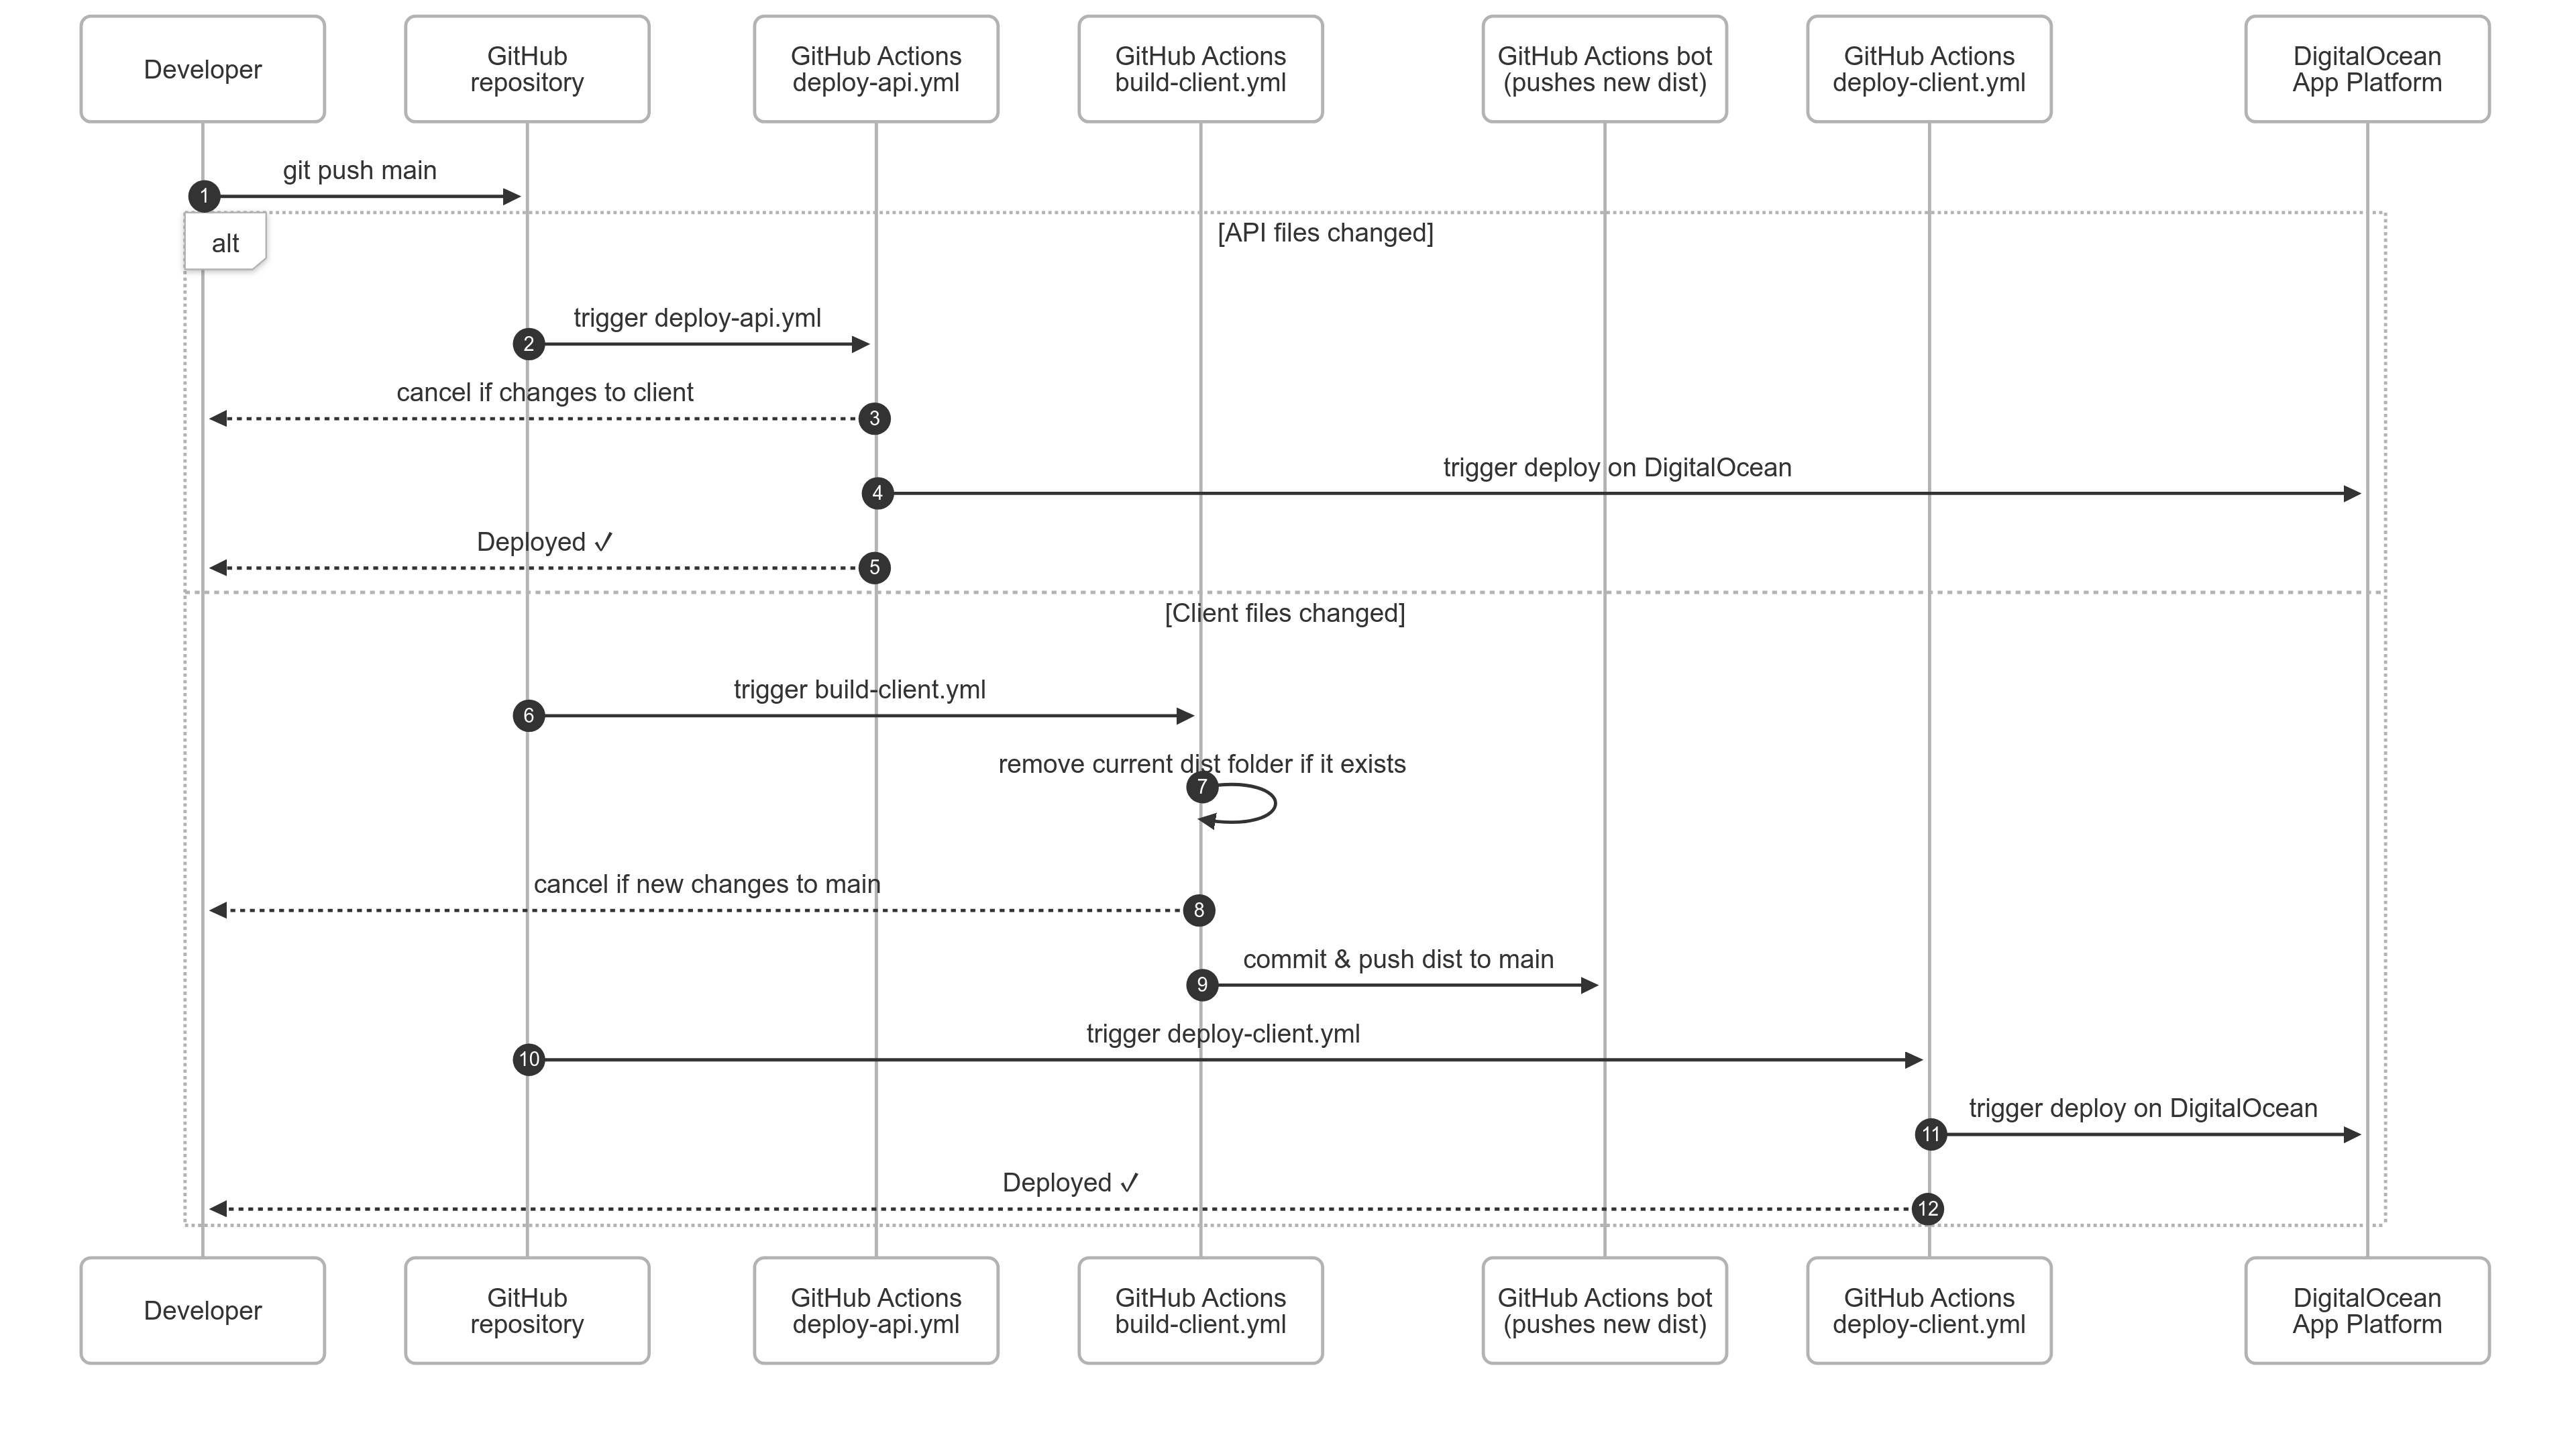
\includegraphics[width=1\linewidth]{images/DeploymentSequence.png}
    \caption{Sequence diagram of the deployment process using GitHub Actions.}
    \label{fig:DeploymentSequence}
\end{figure}

\subsubsection{Scaling \& upgrade strategy}
Our deployment runs on DigitalOcean App Platform, which enables us to apply horizontal scaling, zero-downtime upgrades, and rollbacks.
\\\\
It uses the blue-green rollout strategy. creating a new set of containers, that gets updated and traffic transferred to them. With the option to roll-back upon failure \cite{rollbacks}.
\\\\
Every build pushed by GitHub Actions is tagged with
the Git SHA. This means we can redeploy the previous SHA, instantly restoring the last known-good state.
\\\\
Each container can be monitored for average CPU utilization, meaning the amount of instances running at a time is constantly changing, depending on settings, optimizing our instance utilization \cite{app_scaling}.

\subsection{Monitoring}
At the moment we rely only on the basic CPU/RAM graphs that DigitalOcean App Platform provides. In the future, it would be wise to implement a full monitoring stack. Here we could either use a built-in addon to the App Platform, such as 360 Monitoring, or do the Prometheus + Grafana stack inspired by the course example:

\paragraph{Collection layer (Prometheus)}
\begin{itemize}
  \item \textbf{Application metrics} – expose the built-in
        \lstinline{/metrics} endpoint from ASP.NET Core via the
        \textit{prometheus-net.AspNetCore} package; record
        HTTP~latency, status-code counts, and SignalR connection count.
  \item \textbf{Client metrics} – ship front-end Web Vitals
        (Cumulative Layout Shift, First Input Delay, Largest Contentful Paint) to Prometheus with the
        \textit{@grafana/web-vitals-exporter} script.
  \item \textbf{Infrastructure exporters} – run the
        \textit{mysql\_exporter} for DB metrics
\end{itemize}

\paragraph{Visualisation layer (Grafana)}
\begin{itemize}
  \item Run Grafana in a Docker container and point it at a folder that
        contains dashboard JSON files. When the container restarts it
        automatically reloads the same dashboards.
  \item The main dashboard shows five things side-by-side: request rate,
        error rate, 95th-percentile latency, database queries per second, and
        basic CPU / memory use.
  \item Alert rules as simple YAML files. For example, send an alert if
        the 95th-percentile latency stays above 500-ms for five minutes, or
        if the number of open MySQL connections hits the limit.
\end{itemize}

\paragraph{Benefit}
This stack would give a single place for viewing \emph{application},
\emph{database}, and \emph{host} telemetry, with reproducible dashboards
under version control and alert rules. In practice it would cut mean-time-to-detect and provide data for capacity planning.


\subsection{Logging}
As mentioned earlier, we chose to implement our own log viewer. The API sends lines from the logs to the client, which is loaded 50 lines at a time in a textbox, which loads more when scrolling up. SignalR is used for updating the logs in real time. It can be accessed on the \texttt{/logs} page, only to administrators. An administrator account can be accessed through this login:
\begin{equation}
    helgeandmircea
\end{equation}
\begin{equation}
    sesame0uvr3toi
\end{equation}

\subsection{Security}
Every request to MiniTwit-FS travels over HTTPS, then clears JWT authentication and role checks before it reaches the controllers. All database access flows through Entity Framework Core, which compiles parameterised queries and blocks SQL-injection attempts by design \cite{sql-queries}. User passwords are stored as SHA-256 hashes in the database.\\\\
Sessions ride on HttpOnly cookies that expire after 30 minutes of idle time and work only from whitelisted origins set by CORS. Input DTOs carry data-annotation rules—length limits, required fields, email regexes so malformed payloads are rejected by the client.\\\\
Secrets such as DB credentials and the JWT key stay in environment variables, and any that reach the logs are masked. SnapShooter \cite{snapshooter} takes a full database snapshot every night and keeps a seven-day archive, so we can easily restore data.

\subsubsection{Pentest Tool}
\begin{comment}
    The automated scan we ran with OWASP ZAP \cite{zaproxy} produced thirteen findings, none of them classified as high-risk but three that ZAP marks as medium and therefore merit prompt attention.
    The most important observation is the absence of several security-hardening HTTP headers. Every response served by the API lacks a Content-Security-Policy header. This greatly increases our exposure to stored-XSS attacks. The same responses are also missing an anti-clickjacking header, either X-Frame-Options or the newer frame-ancestors directive, so the site can be embedded in a malicious frame and trick users into clicking invisible UI elements. Finally, ZAP located that it is possible to retrieve the index.html file, which by itself isn't harmful to us, but we should acknowledge that we are not hiding our files properly, and be careful of putting information or secrets there.\\\\
    The remaining seven alerts are marked low or informational.\\\\
    Taken as a whole, the report says our surface is not critically vulnerable but is missing a layer of defensive headers and housekeeping that modern security baselines assume. The immediate fixes are all low-effort middleware changes: add a restrictive CSP (default-src 'self' as a starting point), set X-Frame-Options: DENY, enable HSTS, mark cookies SameSite=Lax, and serve X-Content-Type-Options: nosniff. In parallel we should remove or protect the backup files ZAP discovered. Once those changes are deployed we should rerun ZAP, with the goal to at least drive the high and medium-risk count to zero and leave only informational notes in the report.
\end{comment}
OWASP ZAP \cite{zaproxy} logged 13 issues—three medium risk, none high.
The mediums are all missing headers: Content-Security-Policy, anti-clickjacking (X-Frame-Options/frame-ancestors), and a publicly reachable index.html.
Everything else is low or informational.
Fix with a strict CSP (default-src 'self'), X-Frame-Options: DENY, HSTS, SameSite=Lax, X-Content-Type-Options: nosniff, hide backup files, then rerun ZAP to clear the medium findings.